\documentclass{article}
\usepackage[margin=1in]{geometry}
\usepackage{amsmath}
\usepackage{tikz}

\begin{document}

%===========================================================
% FIGURE 1: sigma > 1 (Strong Substitutes)
%===========================================================
\subsection*{Case $\sigma > 1$ (Strong Substitutes)}
When goods are strong substitutes, a decrease in $l_2$ makes good 2 cheaper, shifting consumption towards $x_2$ and reducing demand for $x_1$. The labor employed in sector 2 ($L_2$) increases, while sector 1 ($L_1$) shrinks.

\begin{figure}[ht]
\centering
{\large \bfseries Case $\sigma > 1$}\\[1em]

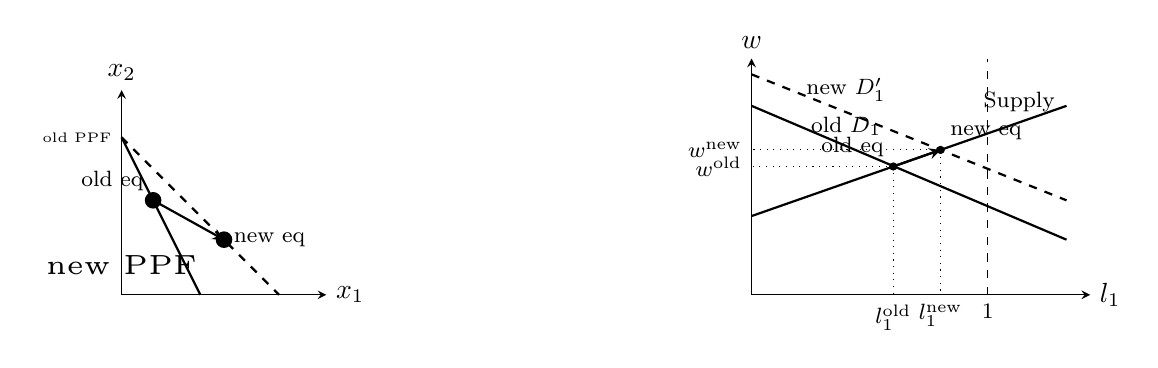
\begin{tikzpicture}[>=stealth]

%------------------ LEFT PANEL (PPF) ------------------%
\begin{scope}[xshift=0cm, yshift=0cm, scale=2.0]
  \draw[->] (0,0) -- (1.3,0) node[right] {$x_{1}$};
  \draw[->] (0,0) -- (0,1.3) node[above] {$x_{2}$};

  % Old PPF (solid)
  \draw[thick]
    (0,1) node[left, font=\tiny]{old PPF}
    -- (0.5,0);

  % New PPF (dashed)
  \draw[thick, dashed]
    (0,1) node[pos=0.5, above, font=\tiny]{new PPF}
    -- (1,0);

  \coordinate (E0) at (0.2,0.6);
  \fill (E0) circle(1.5pt);
  \node[above left, font=\footnotesize] at (E0) {old eq};

  \coordinate (E1) at (0.65,0.35);
  \fill (E1) circle(1.5pt);
  \node[right, font=\footnotesize] at (E1) {new eq};

  \draw[->, thick] (E0) -- (E1);
\end{scope}

%------------------ RIGHT PANEL (Labor Market) ------------------%
\begin{scope}[xshift=8cm, yshift=0cm, scale=1.0]
  \draw[->] (0,0) -- (4.3,0) node[right] {$l_{1}$};
  \draw[->] (0,0) -- (0,3)   node[above] {$w$};

  % vertical line at x=3
  \draw[dashed] (3,0) -- (3,3);
  \node[below, font=\footnotesize] at (3,0) {$1$};

  % Labor supply (solid)
  \draw[thick]
    (0,1) -- (4,2.4)
    node[pos=0.85, above, font=\footnotesize] {Supply};

  % Old labor demand (solid)
  \draw[thick]
    (0,2.4) -- (4,0.7)
    node[pos=0.3, above, font=\footnotesize] {old $D_{1}$};

  % New labor demand (dashed)
  \draw[thick, dashed]
    (0,2.8) -- (4,1.2)
    node[pos=0.3, above, font=\footnotesize] {new $D_{1}'$};

  \coordinate (E0Lm) at (1.8,1.63);
  \fill (E0Lm) circle(1.5pt);
  \node[above left, font=\footnotesize] at (E0Lm) {old eq};

  \coordinate (E1Lm) at (2.4,1.84);
  \fill (E1Lm) circle(1.5pt);
  \node[above right, font=\footnotesize] at (E1Lm) {new eq};

  \draw[->, thick] (E0Lm) -- (E1Lm);

  \draw[dotted] (E0Lm) -- (1.8,0) node[below, font=\footnotesize] {$l_{1}^{\text{old}}$};
  \draw[dotted] (E0Lm) -- (0,1.63) node[left, font=\footnotesize] {$w^{\text{old}}$};
  \draw[dotted] (E1Lm) -- (2.4,0) node[below, font=\footnotesize] {$l_{1}^{\text{new}}$};
  \draw[dotted] (E1Lm) -- (0,1.84) node[left, font=\footnotesize] {$w^{\text{new}}$};
\end{scope}

\end{tikzpicture}

\caption{When goods are strong substitutes ($\sigma>1$), a productivity improvement in good 1 shifts consumption strongly toward $x_1$ and increases sector 1's labor demand and wage. 
Dashed lines represent the after-shock production possibility frontier and new labor demand.}
\end{figure}


\vspace{2cm}
%===========================================================
% FIGURE 2: sigma = 1 (Cobb--Douglas)
%===========================================================
\subsection*{Case $\sigma = 1$ (Cobb--Douglas)}
Under Cobb--Douglas preferences, the consumer spends fixed shares on each good, meaning that $x_1$ remains constant while $x_2$ increases. Sectoral employment remains unchanged.

\begin{figure}[ht]
\centering
{\large \bfseries Case $\sigma = 1$}\\[1em]

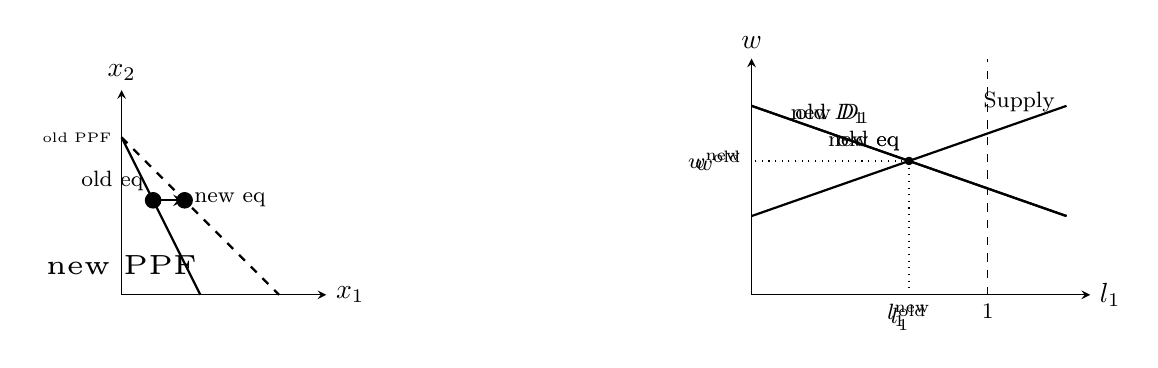
\begin{tikzpicture}[>=stealth]

%------------------ LEFT PANEL (PPF) ------------------%
\begin{scope}[xshift=0cm, yshift=0cm, scale=2.0]
  \draw[->] (0,0) -- (1.3,0) node[right] {$x_{1}$};
  \draw[->] (0,0) -- (0,1.3) node[above] {$x_{2}$};

  \draw[thick] (0,1) node[left, font=\tiny]{old PPF} -- (0.5,0);
  \draw[thick, dashed] (0,1) node[pos=0.5, above, font=\tiny]{new PPF} -- (1,0);

  \coordinate (E0) at (0.2,0.6);
  \fill (E0) circle(1.5pt);
  \node[above left, font=\footnotesize] at (E0) {old eq};

  \coordinate (E1) at (0.4,0.6);
  \fill (E1) circle(1.5pt);
  \node[right, font=\footnotesize] at (E1) {new eq};

  \draw[->, thick] (E0) -- (E1);
\end{scope}

%------------------ RIGHT PANEL (Labor Market) ------------------%
\begin{scope}[xshift=8cm, yshift=0cm, scale=1.0]
  \draw[->] (0,0) -- (4.3,0) node[right] {$l_{1}$};
  \draw[->] (0,0) -- (0,3)   node[above] {$w$};

  \draw[dashed] (3,0) -- (3,3);
  \node[below, font=\footnotesize] at (3,0) {$1$};

  \draw[thick]
    (0,1) -- (4,2.4)
    node[pos=0.85, above, font=\footnotesize] {Supply};
  \draw[thick]
    (0,2.4) -- (4,1.0)
    node[pos=0.25, above, font=\footnotesize] {old $D_{1}$};
  \draw[thick]
    (0,2.4) -- (4,1.0)
    node[pos=0.25, above, font=\footnotesize] {new $D_{1}$};

  \coordinate (E0Lm) at (2,1.7);
  \fill (E0Lm) circle(1.5pt);
  \node[above left, font=\footnotesize] at (E0Lm) {old eq};

  \coordinate (E0Lm) at (2,1.7);
  \fill (E0Lm) circle(1.5pt);
  \node[above left, font=\footnotesize] at (E0Lm) {new eq};



  \draw[dotted] (E0Lm) -- (2,0)   node[below, font=\footnotesize] {$l_{1}^{\text{old}}$};
  \draw[dotted] (E0Lm) -- (0,1.7) node[left, font=\footnotesize] {$w^{\text{old}}$};
  \draw[dotted] (E0Lm) -- (2,0)   node[below, font=\footnotesize] {$l_{1}^{\text{new}}$};
  \draw[dotted] (E0Lm) -- (0,1.7) node[left, font=\footnotesize] {$w^{\text{new}}$};
  \end{scope}

\end{tikzpicture}

\caption{Under Cobb--Douglas preferences ($\sigma=1$), the consumer spends fixed shares on each good, so $x_2$ remains the same while $x_1$ increases. Labor demand in sector 1 rises moderately, pushing up $l_{1}$ and the wage. 
Dashed lines represent the after-shock production possibility frontier and new labor demand.}
\end{figure}


\vspace{2cm}
%===========================================================
% FIGURE 3: sigma < 1 (Complements)
%===========================================================
\subsection*{Case $\sigma < 1$ (Complements)}
When goods are complements, both $x_1$ and $x_2$ increase. Sector 1 expands, drawing labor away from sector 2, so $L_1$ rises and $L_2$ decreases.

\begin{figure}[ht]
\centering
{\large \bfseries Case $\sigma < 1$}\\[1em]

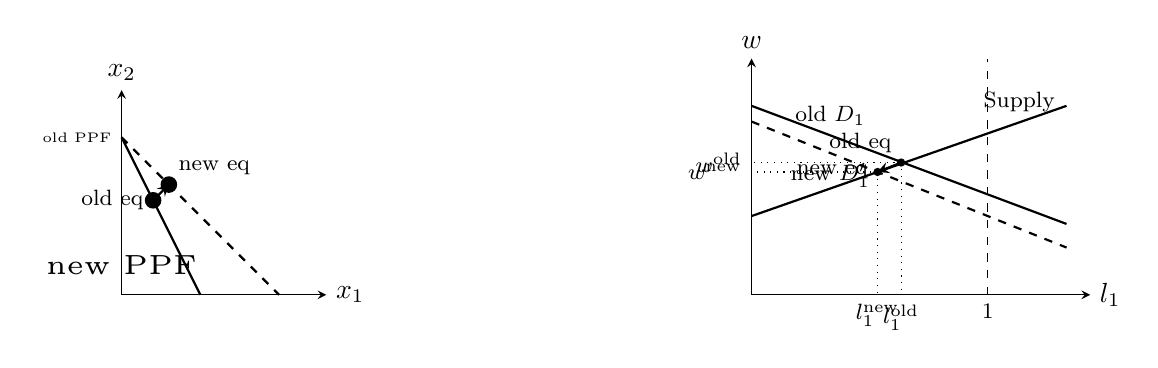
\begin{tikzpicture}[>=stealth]

%------------------ LEFT PANEL (PPF) ------------------%
\begin{scope}[xshift=0cm, yshift=0cm, scale=2.0]
  \draw[->] (0,0) -- (1.3,0) node[right] {$x_{1}$};
  \draw[->] (0,0) -- (0,1.3) node[above] {$x_{2}$};

  \draw[thick]
    (0,1) node[left, font=\tiny]{old PPF}
    -- (0.5,0);
  \draw[thick, dashed]
    (0,1) node[pos=0.5, above, font=\tiny]{new PPF}
    -- (1,0);

  \coordinate (E0) at (0.2,0.6);
  \fill (E0) circle(1.5pt);
  \node[left, font=\footnotesize] at (E0) {old eq};

  \coordinate (E1) at (0.3,0.7);
  \fill (E1) circle(1.5pt);
  \node[above right, font=\footnotesize] at (E1) {new eq};

  \draw[->, thick] (E0) -- (E1);
\end{scope}

%------------------ RIGHT PANEL (Labor Market) ------------------%
\begin{scope}[xshift=8cm, yshift=0cm, scale=1.0]
  \draw[->] (0,0) -- (4.3,0) node[right] {$l_{1}$};
  \draw[->] (0,0) -- (0,3)   node[above] {$w$};

  \draw[dashed] (3,0) -- (3,3);
  \node[below, font=\footnotesize] at (3,0) {$1$};

  \draw[thick]
    (0,1) -- (4,2.4)
    node[pos=0.85, above, font=\footnotesize] {Supply};
  \draw[thick]
    (0,2.4) -- (4,0.9)
    node[pos=0.25, above, font=\footnotesize] {old $D_{1}$};
  \draw[thick, dashed]
    (0,2.2) -- (4,0.6)
    node[pos=0.25, below, font=\footnotesize] {new $D_{1}'$};

  \coordinate (E0Lm) at (1.9,1.68);
  \fill (E0Lm) circle(1.5pt);
  \node[above left, font=\footnotesize] at (E0Lm) {old eq};

  \coordinate (E1Lm) at (1.6,1.56);
  \fill (E1Lm) circle(1.5pt);
  \node[left, font=\footnotesize] at (E1Lm) {new eq};

  \draw[->, thick] (E0Lm) -- (E1Lm);

  \draw[dotted] (E0Lm) -- (1.9,0) node[below, font=\footnotesize] {$l_{1}^{\text{old}}$};
  \draw[dotted] (E0Lm) -- (0,1.68) node[left, font=\footnotesize] {$w^{\text{old}}$};
  \draw[dotted] (E1Lm) -- (1.6,0) node[below, font=\footnotesize] {$l_{1}^{\text{new}}$};
  \draw[dotted] (E1Lm) -- (0,1.56) node[left, font=\footnotesize] {$w^{\text{new}}$};
\end{scope}

\end{tikzpicture}

\caption{When goods are complements ($\sigma<1$), both $x_1$ and $x_2$ rise in consumption, but sector 1's labor demand may decrease if labor-saving dominates, reducing $l_{1}$ and wage $w$. 
Dashed lines represent the after-shock production possibility frontier and new labor demand.}
\end{figure}

\end{document}